\documentclass[border=10pt]{standalone}
\usepackage{pgfplots}
\pgfplotsset{compat=1.18}
\begin{document}
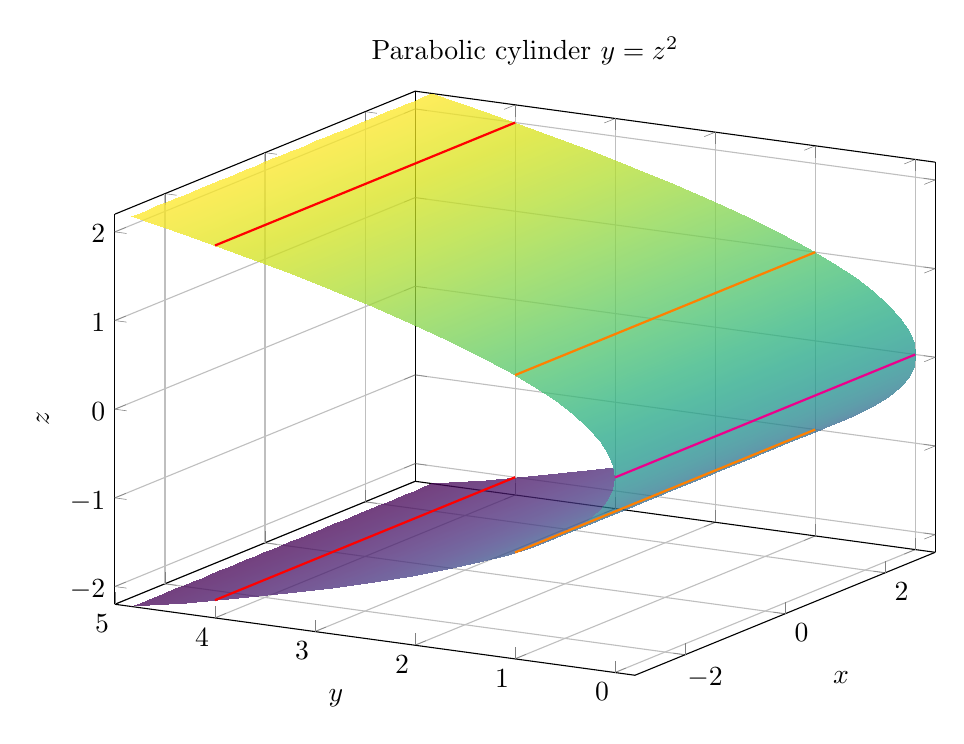
\begin{tikzpicture}
\begin{axis}[
    view={-60}{20},
    xlabel={$x$}, ylabel={$y$}, zlabel={$z$},
    title={Parabolic cylinder $y=z^2$},
    domain=-3:3,
    y domain=-2.2:2.2,
    samples=35,
    samples y=35,
    colormap/viridis,
    width=12cm,
    height=9cm,
    xmin=-3, xmax=3,
    ymin=-0.2, ymax=5,
    zmin=-2.2, zmax=2.2,
    grid=major,
]
\addplot3[surf, opacity=0.75, shader=interp] ({x}, {y^2}, {y});
\addplot3[red, thick, domain=-3:3, samples=100] ({x}, {4}, {-2});
\addplot3[orange, thick, domain=-3:3, samples=100] ({x}, {1}, {-1});
\addplot3[magenta, thick, domain=-3:3, samples=100] ({x}, {0}, {0});
\addplot3[orange, thick, domain=-3:3, samples=100] ({x}, {1}, {1});
\addplot3[red, thick, domain=-3:3, samples=100] ({x}, {4}, {2});
\end{axis}
\end{tikzpicture}
\end{document}